\documentclass[11pt, oneside]{article} 
\usepackage{geometry}
\geometry{letterpaper} 
\usepackage{graphicx}
	
\usepackage{amssymb}
\usepackage{amsmath}
\usepackage{parskip}
\usepackage{color}
\usepackage{hyperref}

\graphicspath{{/Users/telliott/Dropbox/Github-Math/quickgeo/figures/}{/Users/telliott/Dropbox/Github-Math/figures/}}

\title{Pentagon}
\date{}

\begin{document}
\maketitle
\Large

%[my-super-duper-separator]

In this chapter we explore some properties of a regular pentagon.  A pentagon has 5 sides, and a regular polygon has all sides equal.  The regular pentagon has five-fold rotational symmetry.  

Draw all of the internal chords of the figure and label a few angles.  By rotational symmetry each of the five vertices of the pentagon has the same three components, the central one labeled $s$, and two flanking angles $r$ and $t$ (left panel).  
\begin{center} 
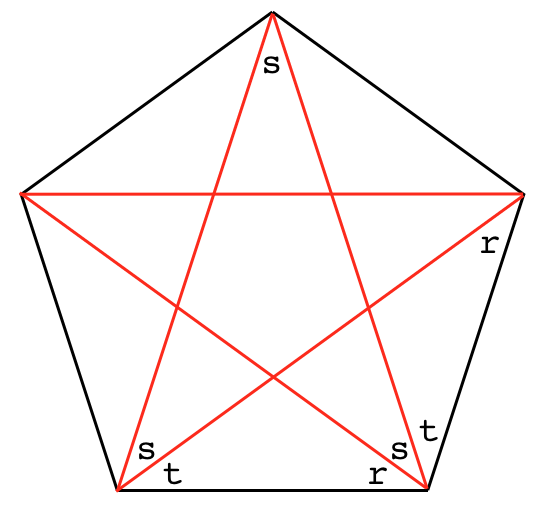
\includegraphics [scale=0.3] {pent1.png}
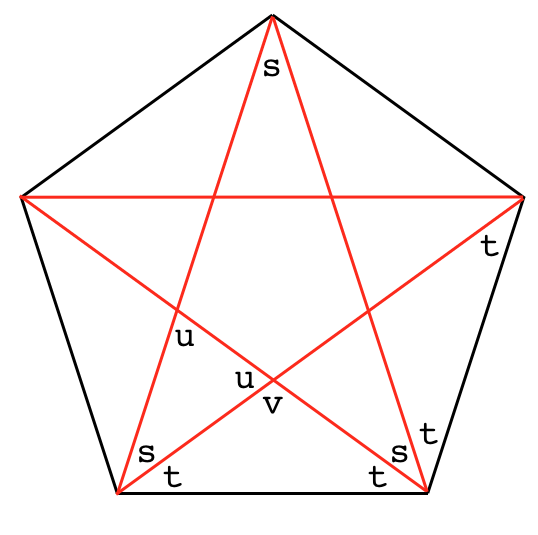
\includegraphics [scale=0.3] {pent2.png} 
\end{center}
First, we observe that the triangle formed with two equal sides at the lower right, has equal base angles by the isosceles triangle theorem.  Therefore $r = t$ (right panel).  

Next, we count up all the angles in two triangles.  In the tall skinny triangle we have $3s + 2t$ while in the short, squat one on the right we have $4t + s$.  But these are equal, by the triangle sum theorem:
\[ 3s + 2t = 4t + s \]

I'm sure you can complete the proof.  $s = t$.  All three angles at each vertex are equal.  We also have that $s$ is one-fifth of $180$, so $s = 36$.  

The central angle subtending each face (not shown) is $2s = 72$.  We can get that by the inscribed angle theorem, since we know $s$, or simply from the five-fold symmetry.

Continuing:
\begin{center}
\includegraphics [scale=0.35] {pent3b.png}
\end{center}

By counting the angles in a triangle again, we conclude that the angles marked with pink dots (e.g. $\angle BPQ$) are equal to two copies of $s$.  We conclude that $AC \parallel ED$ by the converse of alternate interior angles. 

The chord above the base that looks like it's parallel \emph{is} parallel.  The parallelograms inside the figure like $PCED$ are actually rhombi, with all sides equal, since opposite sides of a parallelogram are equal.

All this means that we have two sets of similar triangles, as well as a small pentagon at the center.  $\triangle BPQ \sim \triangle BED$ and $\triangle ABE \sim \triangle ABP$.

Here are three examples of the tall skinny type:
\begin{center} \includegraphics [scale=0.4] {three_triangles_2.png} \end{center}

Suppose we scale things so the base of the skinny blue triangle is $1$ and the side of the pentagon is $x$.  Then, for the tall skinny red triangle the ratio of sides is $(x + 1)/x$ and for the blue one it's $x/1$.  This gives
\[ \frac{x + 1}{x} = x \]
\[ x^2 = x + 1 \]
We won't solve this equation here, but just give the result.

$x$ is usually called $\phi$, the famous \emph{golden mean} or golden ratio:
\[ \phi = \frac{1}{2} (1 + \sqrt{5}) \]

We should check that $\phi$ really does solve the equation:
\[ \phi^2 =  \frac{1}{4} (1 + \sqrt{5})^2 \]
\[ = \frac{1}{4} (1 + 2 \sqrt{5} + 5) \]
\[ = \frac{1}{4} (6 + 2 \sqrt{5} ) \]
\[ = 1 + \phi \]

\subsection*{golden mean}

One way to introduce the golden ratio is to take an arbitrary length and pick a point on it, dividing the whole into one part of length $a$ and the other of length $b$.  Suppose $a$ is greater than $b$.
\begin{center} 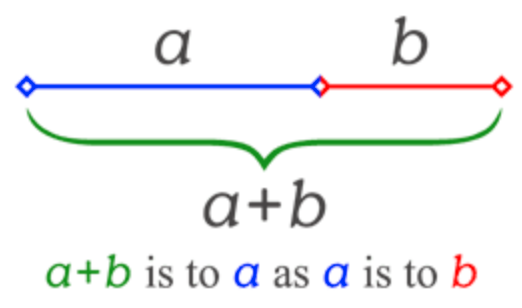
\includegraphics [scale=0.5] {golden_ratio.png} \end{center}
Then, the definition of the golden ratio $a:b$ is
\[ \frac{a + b}{a} = \frac{a}{b} \]
The ratio of the whole length to $a$  is the same as the ratio of $a$ to $b$.

We can do a similar trick with rectangles.
\begin{center} 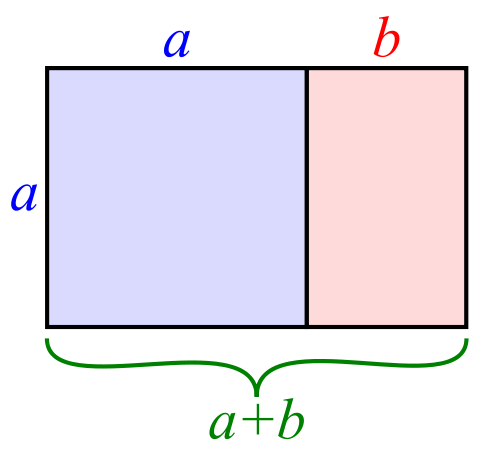
\includegraphics [scale=0.3] {goldenratioab.png} \end{center}
Draw a square with sides $a$, and extend it a distance $b$ to form a rectangle of side length $a + b$.  We want the proportions of the two rectangles in the figure to be the equal, and this gives the same equation as before.

Going back to that equation, since the length is arbitrary, we can scale it so $b = 1$.
\[ a = \frac{a + 1}{a} \]
\[ a^2 = a + 1 \]
This is exactly what we had above.

\subsection*{construction}

It is quite a challenge to construct a pentagon freehand.  Some very interesting methods using ruler and compass are given in wikipedia

\url{https://en.wikipedia.org/wiki/Pentagon}

Here is a third one.  

\url{https://www.goldennumber.net/phi-formula-geometry}

We first construct the length 
\[ \phi = \frac{1}{2} (1 + \sqrt{5}) \]
Draw 3 identical circles of diameter $1$ next to each other.  It might help to first construct a rectangle with sides of length $2$ and $1/2$ and subdivide the length into two parts, in order to place the centers and bases in the right orientation.
\begin{center} 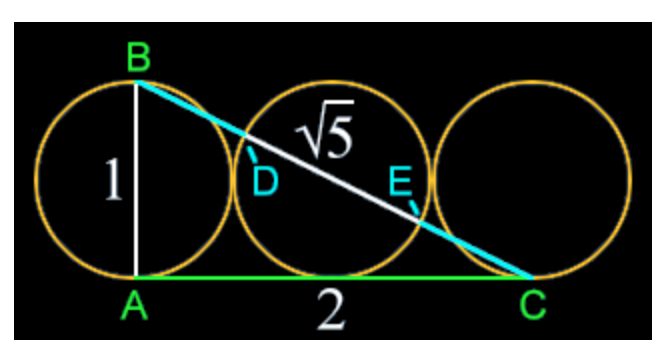
\includegraphics [scale=0.5] {phi_construct.png} \end{center}

Find the base point at $C$ and connect $BC$.  The Pythagorean theorem gives us that $BC = \sqrt{5}$.  So from $B$ to the center of the middle circle is one-half that, and extending along the line to the point $E$ adds another $1/2$.  We have
\[ BE = \frac{\sqrt{5}}{2} + \frac{1}{2} \]
which, with a slight rearrangement, can be seen to be equal to $\phi$.

So now we have the length $\phi$, based on a given length $1$.  Go back to the tall skinny red triangle:
\begin{center} \includegraphics [scale=0.4] {three_triangles_2.png} \end{center}

To duplicate this, mark off a length $1$ for the base.  Then find the intersection of two arcs of length $\phi$, putting one pin of the compass on each endpoint of the base.  This fixes the top vertex.  

Finally, mark off arcs of length $1$ from the top and the sides of the base to place the other two vertices.

\subsection*{Brief aside on $\phi$ and the Fibonacci sequence}

$\phi \approx 1.618$.

The Fibonacci sequence is defined as $F_{n} = F_{n-1} + F_{n-2}$, starting with $1,1$ as the first two numbers.

The first ten numbers in the sequence are:
\begin{verbatim}
1 1 2 3 5 8 13 21 34 55 ...
\end{verbatim}

As the numbers in the Fibonacci sequence get larger, the ratio $F_{n} / F_{n-1}$ becomes a better and better approximation to $\phi$.  Binet's formula turns this around and uses $\phi$ to calculate the nth Fibonacci number.

Here is some Python code to give large values of $F_n$ and calculate the ratio $F_{n} / F_{n-1}$:
\begin{verbatim}
>>> phi = (1 + 5**0.5)/2
>>> phi
1.618033988749895
>>>
>>> def f(n):
...     a,b = 1,1
...     for i in range(n):
...         a,b = a+b, a
...     return a,b,a/b
... 
>>> f(10)
(144, 89, 1.6179775280898876)
>>> f(30)
(2178309, 1346269, 1.6180339887496482)
>>> 
\end{verbatim}

(This code relies on the fact that the value of $a$ is cached for the tuple assignment a,b = a+b, a). It should be clear that $F_n/F_{n-1}$ becomes a better and better approximation to $\phi$ as it gets larger.

\subsection*{irrationality}

$\phi$ is an \emph{irrational} number, a concept that gave the Greeks fits.

This means that it cannot be written as the ratio of two integers, and what amounts to the same thing, an accurate decimal representation goes on forever.

One way to see this is to construct the continued fraction representation of $\phi$.
\[ \phi^2 = \phi + 1 \]
Dividing by $\phi$ we get
\[ \phi = 1 + \frac{1}{\phi} \]

The trick here is to see that the \emph{entire} right-hand side of the equation above is equal to $\phi$ so that whole thing can be substituted for the denominator of the second term on that side.
\[ \phi = 1 + \frac{1}{1 + \frac{1}{\phi}} \]

This goes on forever.
\[ \phi = 1 + \cfrac{1}{1+\cfrac{1}{1+\cfrac{1}{1 + \dots}}}  \]

Those dots mean that to evaluate this expression, at some point we must decide to neglect the remaining terms.  If we take a finite number of terms, there will always be some error between what we calculate and the true value of $\phi$.   

Going back up the chain, we start with by ignoring the dots to get $1$ and then repeatedly add one, invert, add one, invert, etc.

\begin{verbatim}
1 + 1 = 2
1/2 + 1 = 3/2
2/3 + 1 = 5/3
3/5 + 1 = 8/5
5/8 + 1 = 13/8
\end{verbatim}

Can you see the Fibonacci sequence developing?

\end{document}